
% Copyright 2004 by Till Tantau <tantau@users.sourceforge.net>.
%
% In principle, this file can be redistributed and/or modified under
% the terms of the GNU Public License, version 2.
%
% However, this file is supposed to be a template to be modified
% for your own needs. For this reason, if you use this file as a
% template and not specifically distribute it as part of a another
% package/program, I grant the extra permission to freely copy and
% modify this file as you see fit and even to delete this copyright
% notice. 

\documentclass[pdf]{beamer}
\mode<presentation>{}

\usepackage[utf8]{inputenc}
\usepackage{amssymb}
\usepackage{amsmath}
\usepackage{graphicx}


% There are many different themes available for Beamer. A comprehensive
% list with examples is given here:
% http://deic.uab.es/~iblanes/beamer_gallery/index_by_theme.html
% You can uncomment the themes below if you would like to use a different
% one:
%\usetheme{AnnArbor}
%\usetheme{Antibes}
%\usetheme{Bergen}
%\usetheme{Berkeley}
%\usetheme{Berlin}
%\usetheme{Boadilla}
%\usetheme{boxes}
%\usetheme{CambridgeUS}
\usetheme{Copenhagen}
%\usetheme{Darmstadt}
%\usetheme{default}
%\usetheme{Frankfurt}
%\usetheme{Goettingen}
%\usetheme{Hannover}
%\usetheme{Ilmenau}
%\usetheme{JuanLesPins}
%\usetheme{Luebeck}
%\usetheme{Madrid}
%\usetheme{Malmoe}
%\usetheme{Marburg}
%\usetheme{Montpellier}
%\usetheme{PaloAlto}
%\usetheme{Pittsburgh}
%\usetheme{Rochester}
%\usetheme{Singapore}
%\usetheme{Szeged}
%\usetheme{Warsaw}
%\usecolortheme{seahorse}


\title{Orthogonal Range Searching in $2$D\\ using Ball Inheritance}
\author{Mads Ravn}
\institute{Computer Science, Aarhus University}
\date{2015}
 
\pgfdeclareimage[height=0.5cm]{university-logo}{logo-eps-converted-to.pdf}
\logo{\pgfuseimage{university-logo}}

% Delete this, if you do not want the table of contents to pop up at
% the beginning of each subsection:
\AtBeginSubsection[]
{
  \begin{frame}<beamer>{Outline}
    \tableofcontents[currentsection,currentsubsection]
  \end{frame}
}

% Let's get started
\begin{document}

\begin{frame}
  \titlepage
\end{frame}

\begin{frame}{Outline}
  \tableofcontents
  % You might wish to add the option [pausesections]
\end{frame}

\section{Introduction}
\subsection{Orthogonal Range Searching}

\begin{frame}{Orthogonal Range Searching}
  \frametitle{Orthogonal Range Searching}
  \begin{center}
    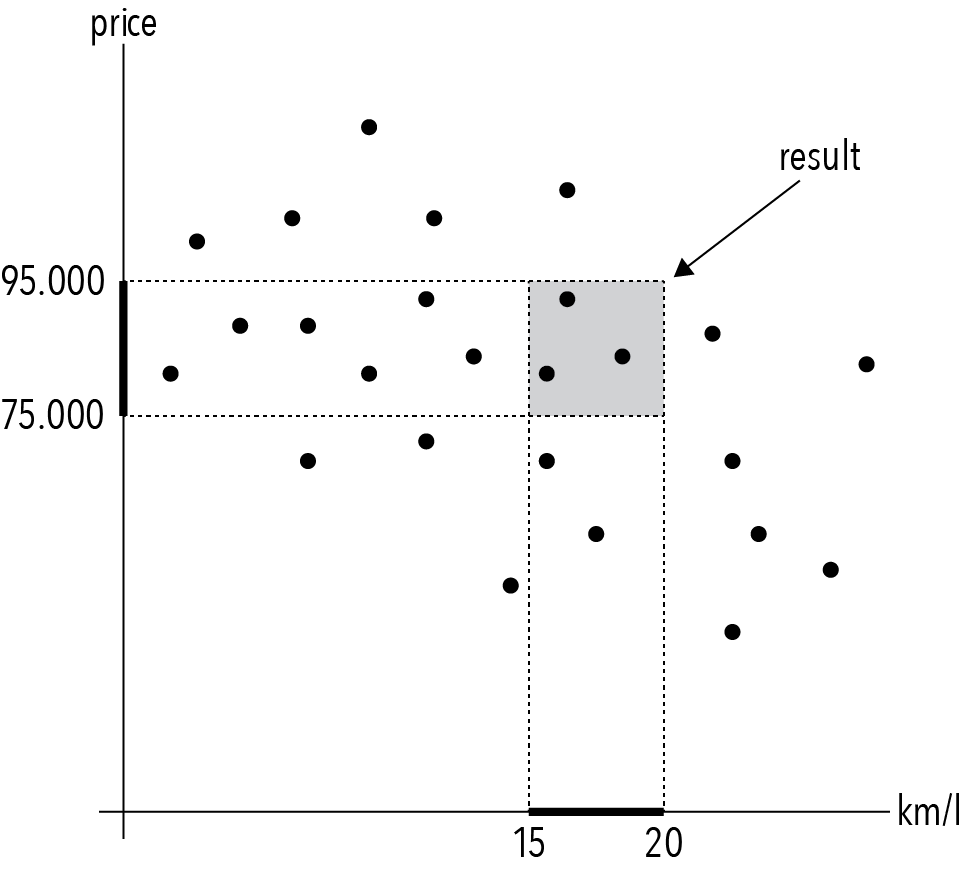
\includegraphics{pictures/introduction.png}
  \end{center}
\end{frame}

\begin{frame}{Preleminaries}
  \frametitle{Preleminaries}
  \begin{itemize}
    \item Alle koordinater er unikke
    \item Rank space
    \item $n$ er en potens af $2$
  \end{itemize}
\end{frame}

\begin{frame}{Orthogonal Range Searching}
  \frametitle{Orthogonal Range Searching}

  Vi er givet $n$ punkter fra $\mathbb{R}^2$ som vi ønsker at indsætte i en datastruktur sådan at vi kan svare effektivt på forespørgslen $q = [x_1, x_2] \times [y_1, y_2]$.
  Et punkt $p = (p_x, p_y)$ ligger i $q = [x_1, x_2] \times [y_1, y_2]$ hvis $p_x \in [x_1, x_2]$ og $p_y \in [y_1, y_2]$. Man kunne derfor sige at et 2-dimensionelt query består af to 1-dimensional sub-queries. Kommer til at virke for alle tre datastrukturer.
\end{frame}

\subsection{Previous data structures}

\begin{frame}{kd-træ}
  \frametitle{kd-træ}
  \textbf{kd-træ}
  \begin{itemize}
    \item $\mathcal{O}(n)$ plads
    \item $\mathcal{O}(\sqrt{n} + k)$ tid
  \end{itemize}
  Givet $n$ punkter: Punkterne bliver sorteret efter $x$ eller $y$ på skift. Median bliver fundet og punkterne mindre end medianen bliver givet til venstre barn og punkterne højere end medianen bliver givet til højre barn. Et punkt per blad i træet.
\end{frame}

\begin{frame}{Opbygning}
  \frametitle{Opbygning af kd-træ}
  Det $\lceil \frac{n}{2} \rceil$'te element bliver valgt som median. Dette element fungerer som en skille-linje mellem de to punkt-mængder. Medianen bliver låst fast på denne plads i arrayet.
  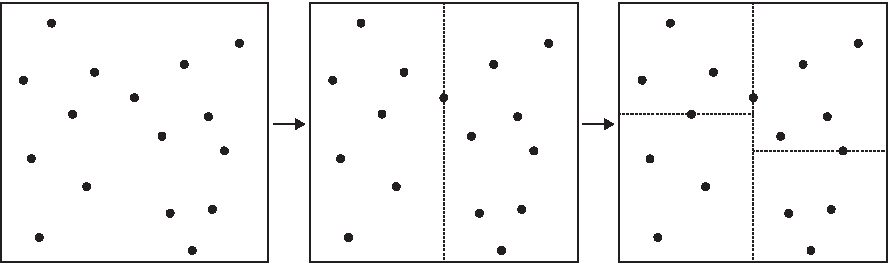
\includegraphics[scale=0.75]{pictures/kd_subdivision-eps-converted-to.pdf}
\end{frame}


\begin{frame}{Søgning}
  \frametitle{Søgning i kd-træ}
  \begin{center}
    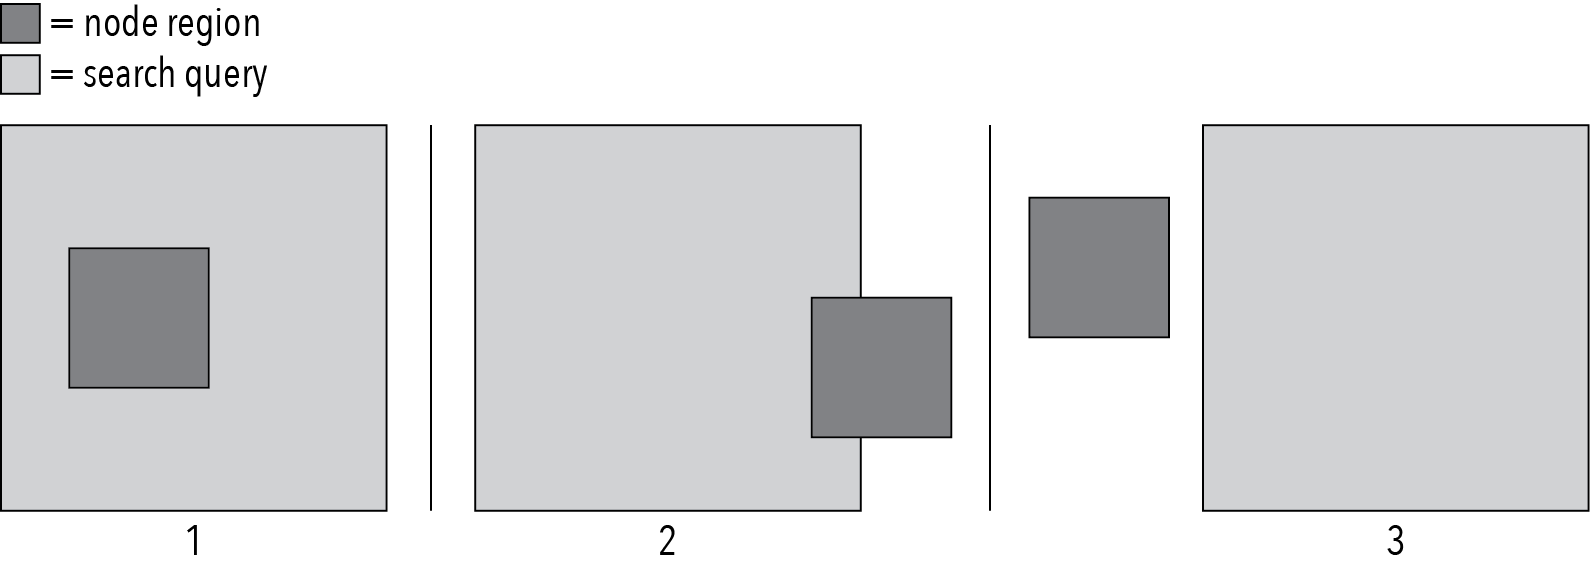
\includegraphics[scale=0.75]{pictures/search_query_overlap.png}
  \end{center}
\end{frame}


% Section and subsections will appear in the presentation overview
% and table of contents.

\section{Ball Inheritance Search}
\begin{frame}{BISintro}
  Ball Inheritance Search, BIS, er en datastruktur bygget som en simplificering af den datastruktur chanetal laver i ARTIKEL

\end{frame}


\subsection{Ball Inheritance Problem}

\begin{frame}{Ball Inheritance}

  \begin{itemize}
    \item Vi er givet et perfekt balanceret søgetræ.
      \pause
    \item Roden indeholder $n$ punkter(bolde) som er blevet fordelt sådan at hvert blad lagrer et punkt.
      \pause
    \item Hver knude har en liste over hvilke af de bolde der er gået igennem den som er blevet givet til venstre og højre barn.
      \pause
    \item Vi kan nu følge en bold fra en knude til et blad med $\mathcal{O}(\lg n)$ skridt.
      \pause
    \item Det er $n \cdot \lg n$ bits plads.
      \pause
    \item Løs: Givet en knude og et index i knudens liste, hvilket blad ender denne bold ved? Vi kan følge bolden 
  \end{itemize}
\end{frame}

\begin{frame}{Faster Queries}
  Vi ønsker at gøre antallet skridt fra en knude til et blad mindre. Vi udvider alfabetet på udvalgte niveauer.
  Vis koncept, tid og plads her
\end{frame}

\begin{frame}{LCA}
  Vis hvordan LCA virker og hvordan vi går ned og hvordan vi finder alle punkter mellem $[x_1, x_2]$.
\end{frame}

\begin{frame}{yrange}
  Vis hvordan vi finder den korrekt y-range. Og hov, det her er jo netop det information vi skal bruge for at løse ball inheritance
\end{frame}

\subsection{Ball Inheritance Search Data Structure}
\begin{frame}{Ball Inheritance Search}
  \textbf{Ball Inheritance Search Data Structure}
  \begin{itemize}
    \item $\mathcal{O}(n)$ plads
    \item $\mathcal{O}(\lg n + k\cdot\lg^\epsilon n)$ tid, hvor $\epsilon > 0$ er en arbitrær lille konstant
  \end{itemize}
\end{frame}

\end{document}


